%%%%%%%%%%%%%%%%%%%%%%%%%%%%%%%%%%%%%%%%%
% Jacobs Landscape Poster
% LaTeX Template
% Version 1.0 (29/03/13)
%
% Created by:
% Computational Physics and Biophysics Group, Jacobs University
% https://teamwork.jacobs-university.de:8443/confluence/display/CoPandBiG/LaTeX+Poster
% 
% Further modified by:
% Nathaniel Johnston (nathaniel@njohnston.ca)
%
% This template has been downloaded from:
% http://www.LaTeXTemplates.com
%
% License:
% CC BY-NC-SA 3.0 (http://creativecommons.org/licenses/by-nc-sa/3.0/)
%
%%%%%%%%%%%%%%%%%%%%%%%%%%%%%%%%%%%%%%%%%
%---------------------------------------------------------------------
%   CONFIGURACION GENERAL
%---------------------------------------------------------------------
\documentclass[final]{beamer}
\usepackage[scale=1.24]{beamerposter} % Use the beamerposter package for laying out the poster
\usetheme{confposter} % Use the confposter theme supplied with this template

%Configurando secciones ['Cuadros de texto' pa los cuates] hay de dos tipos
%1) El puro texto (Sin un marco)
\setbeamercolor{block title}{fg=purple,bg=white} % Bloques (Sin cuadro) - Titulo
\setbeamercolor{block body}{fg=black,bg=white} % Bloques - cuerpo
%2) El texto con marco
\setbeamercolor{block alerted title}{fg=white,bg=dblue!70} % Cuadros - Titulo
\setbeamercolor{block alerted body}{fg=black,bg=dblue!10} % Cuadros - Cuerpo

%-----------------------------------------------------------
% MEDIDAS DEL POSTER
%----------------------------------------------------------
% To set effective sepwid, onecolwid and twocolwid values, first choose how many columns you want and how much separation you want between columns
% In this template, the separation width chosen is 0.024 of the paper width and a 4-column layout
% onecolwid should therefore be (1-(# of columns+1)*sepwid)/# of columns e.g. (1-(4+1)*0.024)/4 = 0.22
% Set twocolwid to be (2*onecolwid)+sepwid = 0.464
% Set threecolwid to be (3*onecolwid)+2*sepwid = 0.708

\newlength{\sepwid}
\newlength{\onecolwid}
\newlength{\twocolwid}
\newlength{\threecolwid}
\setlength{\paperwidth}{78.74in} % Width 198 cm
\setlength{\paperheight}{47.244in} % Heighth 109.22
\setlength{\sepwid}{0.024\paperwidth} % Separation width (white space) between columns
\setlength{\onecolwid}{0.22\paperwidth} % Width of one column
\setlength{\twocolwid}{0.464\paperwidth} % Width of two columns
\setlength{\threecolwid}{0.708\paperwidth} % Width of three columns
\setlength{\topmargin}{0in} % Reduce the top margin size
%-----------------------------------------------------------
% PAQUETES PA' HACER EL POSTER
%-------------------------------------------

\usepackage{graphicx}  % Required for including images
\usepackage[utf8]{inputenc}
\usepackage[portuges, brazil]{babel}   
\usepackage{booktabs} % Top and bottom rules for tables

%----------------------------------------------------------------------------------------
%   TITULO & LOGOS
%----------------------------------------------------------------------------------------

\title{The Mirror Effect within Perception: Not another Recognition Memory Study} % Poster title
\author{Adriana F. Chávez De la Peña} % Author(s)
\institute{National Autonomous University of Mexico (UNAM); Faculty of Psychology\\ Lab 25;  PAPIIT IN307214 - PAPIME PE310016} % Institution(s)

\begin{document}
\addtobeamertemplate{block end}{}{\vspace*{1.5ex}} % White space under blocks
\addtobeamertemplate{block alerted end}{}{\vspace*{1.5ex}} % White space under highlighted (alert) blocks
\setlength{\belowcaptionskip}{2ex} % White space under figures
\setlength\belowdisplayshortskip{2ex} % White space under equations
\begin{frame}[t] % The whole poster is enclosed in one beamer frame
\begin{tikzpicture}[remember picture,overlay]
\node[anchor=north west] at ([shift={(5cm,-1cm)}]current page.north west)
    {
\includegraphics[width=10cm]{Figures/UNAMiwi.jpg}};
\node[anchor=north west] at ([shift={(23cm,-2cm)}]current page.north west)
    {
\includegraphics[width=10cm]{Figures/Psicologia.png}};
\node[anchor=north east] at ([shift={(-15cm,-1cm)}]current page.north east)
    {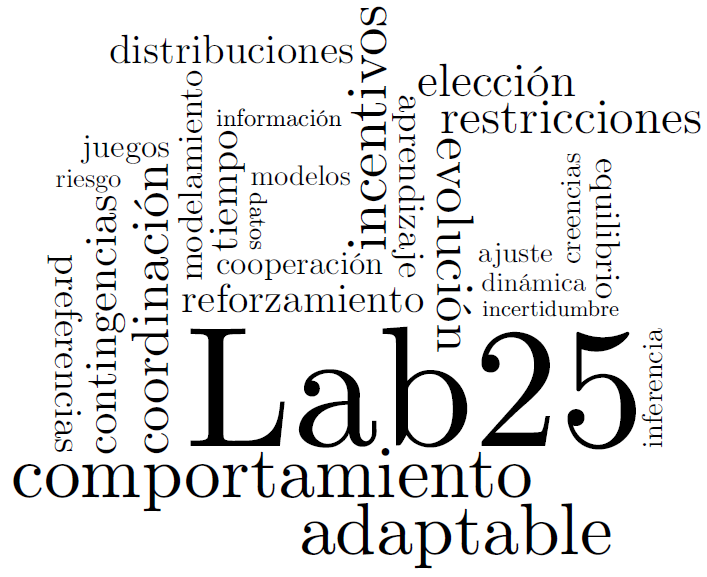
\includegraphics[width=12cm]{Figures/Lab25.png}};
\end{tikzpicture}

%-----------------------------------------------------------------------------------------
%----------------------------------------------------------------------------------------
%   PRIMERA COLUMNA
%----------------------------------------------------------------------------------------
%   INTRODUCCION
%-------------------------------|||

\begin{columns}[t] % The whole poster consists of three major columns, the second of which is split into two columns twice - the [t] option aligns each column's content to the top
\begin{column}{\sepwid}\end{column} % Empty spacer column
\begin{column}{\onecolwid} % The first column

\setbeamercolor{block alerted title}{fg=white,bg=GreenYellow} % Titulo del cuadro
\setbeamercolor{block alerted body}{fg=black,bg=white} % Cuerpo / Contenido del cuadro
\begin{alertblock}{GreenYellow}

Green Yellow
 
\end{alertblock}


\setbeamercolor{block alerted title}{fg=white,bg=Yellow} % Titulo del cuadro
\setbeamercolor{block alerted body}{fg=black,bg=white} % Cuerpo / Contenido del cuadro
\begin{alertblock}{Yellow}

Yellow
 
\end{alertblock}


\setbeamercolor{block alerted title}{fg=white,bg=Goldenrod} 
\setbeamercolor{block alerted body}{fg=black,bg=white} % Cuerpo / Contenido del cuadro
\begin{alertblock}{Goldenrod}

Goldenrod
 
\end{alertblock}


\setbeamercolor{block alerted title}{fg=white,bg=Apricot} 
\setbeamercolor{block alerted body}{fg=black,bg=white} % Cuerpo / Contenido del cuadro
\begin{alertblock}{Apricot}
Apricot
 
\end{alertblock}


\setbeamercolor{block alerted title}{fg=white,bg=Dandelion} % Titulo del cuadro
\setbeamercolor{block alerted body}{fg=black,bg=white} % Cuerpo / Contenido del cuadro
\begin{alertblock}{Dandelion}

Dandelion
 
\end{alertblock}





\setbeamercolor{block alerted title}{fg=white,bg=Peach} % Titulo del Cuadro
\setbeamercolor{block alerted body}{fg=black,bg=white} % Cuerpo / Contenido del cuadro
\begin{alertblock}{Peach}
 Peach

\end{alertblock}



\setbeamercolor{block alerted title}{fg=white,bg=YellowOrange} % Titulo del cuadro
\setbeamercolor{block alerted body}{fg=black,bg=white} % Cuerpo / Contenido del cuadro
\begin{alertblock}{YellowOrange}

YellowOrange
 
\end{alertblock}


\setbeamercolor{block alerted title}{fg=white,bg=BurntOrange} % Titulo del cuadro
\setbeamercolor{block alerted body}{fg=black,bg=white} % Cuerpo / Contenido del cuadro
\begin{alertblock}{BurntOrange}
Burnt Orange
\end{alertblock}



\setbeamercolor{block alerted title}{fg=white,bg=Bittersweet} % Titulo del cuadro
\setbeamercolor{block alerted body}{fg=black,bg=white} % Cuerpo / Contenido del cuadro
\begin{alertblock}{Bittersweet}

Aquamarine 
 
\end{alertblock}



\setbeamercolor{block alerted title}{fg=white,bg=Mahogany} % Titulo del cuadro
\setbeamercolor{block alerted body}{fg=black,bg=white} % Cuerpo / Contenido del cuadro
\begin{alertblock}{Mahogany}

Mahogany
 
\end{alertblock}





\setbeamercolor{block alerted title}{fg=white,bg=BrickRed} % Titulo del cuadro
\setbeamercolor{block alerted body}{fg=black,bg=white} % Cuerpo / Contenido del cuadro
\begin{alertblock}{BrickRed}

BrickRed
 
\end{alertblock}



\setbeamercolor{block alerted title}{fg=white,bg=Red} % Titulo del cuadro
\setbeamercolor{block alerted body}{fg=black,bg=white} % Cuerpo / Contenido del cuadro
\begin{alertblock}{Red}

RED
 
\end{alertblock}




\setbeamercolor{block alerted title}{fg=white,bg=RubineRed} % Titulo del cuadro
\setbeamercolor{block alerted body}{fg=black,bg=white} % Cuerpo / Contenido del cuadro
\begin{alertblock}{RubineRed}

Rubine Red
 
\end{alertblock}





%-----------------------------------------------------------------------------------------
% FIN PRIMERA COLUMNA
%-----------------------------------------------------------------------------------------

\end{column} % End of the first column

\begin{column}{\sepwid}\end{column} % Empty spacer column

\begin{column}{\twocolwid} % Begin a column which is two columns wide (column 2)

%-------------------------------||||||||
\begin{columns}[t,totalwidth=\twocolwid] % Split up the two columns wide column
\begin{column}{\onecolwid}\vspace{-.6in} % The first column within column 2 (column 2.1)

\setbeamercolor{block alerted title}{fg=white,bg=WildStrawberry} % Titulo
\setbeamercolor{block alerted body}{fg=black,bg=white} % Cuerpo
\begin{alertblock}{Orchid}

Wild Strawberry
\end{alertblock}



\setbeamercolor{block alerted title}{fg=white,bg=Salmon} % Titulo
\setbeamercolor{block alerted body}{fg=black,bg=white} % Cuerpo
\begin{alertblock}{Salmon}

Salmon
\end{alertblock}



\setbeamercolor{block alerted title}{fg=white,bg=CarnationPink} % Titulo
\setbeamercolor{block alerted body}{fg=black,bg=white} % Cuerpo
\begin{alertblock}{Carnation Pink}

Carnation Pink
\end{alertblock}



\setbeamercolor{block alerted title}{fg=white,bg=Magenta} % Titulo
\setbeamercolor{block alerted body}{fg=black,bg=white} % Cuerpo
\begin{alertblock}{Magenta}

Magenta
\end{alertblock}




\setbeamercolor{block alerted title}{fg=white,bg=VioletRed} % Titulo
\setbeamercolor{block alerted body}{fg=black,bg=white} % Cuerpo
\begin{alertblock}{VioletRed}

Violet Red
\end{alertblock}




\setbeamercolor{block alerted title}{fg=white,bg=Rhodamine} % Titulo
\setbeamercolor{block alerted body}{fg=black,bg=white} % Cuerpo
\begin{alertblock}{Rhodamine}

Rhodamine
\end{alertblock}



\setbeamercolor{block alerted title}{fg=white,bg=Orchid} % Titulo
\setbeamercolor{block alerted body}{fg=black,bg=white} % Cuerpo
\begin{alertblock}{Orchid}

Orchid
\end{alertblock}




\setbeamercolor{block alerted title}{fg=white,bg=Thistle} % Titulo
\setbeamercolor{block alerted body}{fg=black,bg=white} % Cuerpo
\begin{alertblock}{Thistle}

Thistle
\end{alertblock}


\setbeamercolor{block alerted title}{fg=white,bg=DarkOrchid} % Titulo
\setbeamercolor{block alerted body}{fg=black,bg=white} % Cuerpo
\begin{alertblock}{DarkOrchid}

Dark Orchid
\end{alertblock}



\setbeamercolor{block alerted title}{fg=white,bg=Purple} % Titulo
\setbeamercolor{block alerted body}{fg=black,bg=white} % Cuerpo
\begin{alertblock}{Purple}

Purple
\end{alertblock}


\setbeamercolor{block alerted title}{fg=white,bg=Plum} % Titulo
\setbeamercolor{block alerted body}{fg=black,bg=white} % Cuerpo
\begin{alertblock}{Plum}

Plum
\end{alertblock}


\setbeamercolor{block alerted title}{fg=white,bg=RoyalPurple} % Titulo
\setbeamercolor{block alerted body}{fg=black,bg=white} % Cuerpo
\begin{alertblock}{RoyalPurple}

RoyalPurple
\end{alertblock}



\setbeamercolor{block alerted title}{fg=white,bg=Periwinkle} % Titulo
\setbeamercolor{block alerted body}{fg=black,bg=white} % Cuerpo
\begin{alertblock}{Periwinkle}

Periwinkle
\end{alertblock}






\end{column} % End of column 2.1
%----------------------------------------------------------------------------------------

%----------------------------------------------------------------------------------------
%   BAYESIAN MODELING 
%----------------------------------------------------------------------------------------
\begin{column}{\sepwid}\end{column} % Empty spacer column
\begin{column}{\onecolwid}\vspace{-2.1in} % The second column within column 2 (column 2.2)


\begin{itemize}
\item
\item
\end{itemize}

\setbeamercolor{block alerted title}{fg=white,bg=CadetBlue} % Titulo
\setbeamercolor{block alerted body}{fg=black,bg=white} % Cuerpo
\begin{alertblock}{CadetBlue}

Cadet Blue
\end{alertblock}



\setbeamercolor{block alerted title}{fg=white,bg=CornflowerBlue} % Titulo
\setbeamercolor{block alerted body}{fg=black,bg=white} % Cuerpo
\begin{alertblock}{CornflowerBlue}

Cornflower Blue
\end{alertblock}




\setbeamercolor{block alerted title}{fg=white,bg=MidnightBlue} % Titulo
\setbeamercolor{block alerted body}{fg=black,bg=white} % Cuerpo
\begin{alertblock}{MidnightBlue}

MidnightBlue
\end{alertblock}



\setbeamercolor{block alerted title}{fg=white,bg=NavyBlue} % Titulo
\setbeamercolor{block alerted body}{fg=black,bg=white} % Cuerpo
\begin{alertblock}{NavyBlue}

Navy Blue
\end{alertblock}



\setbeamercolor{block alerted title}{fg=white,bg=RoyalBlue} % Titulo
\setbeamercolor{block alerted body}{fg=black,bg=white} % Cuerpo
\begin{alertblock}{RoyalBlue}

Royal Blue
\end{alertblock}




\setbeamercolor{block alerted title}{fg=white,bg=Blue} % Titulo
\setbeamercolor{block alerted body}{fg=black,bg=white} % Cuerpo
\begin{alertblock}{Blue}

Blue
\end{alertblock}




\setbeamercolor{block alerted title}{fg=white,bg=Cerulean} % Titulo
\setbeamercolor{block alerted body}{fg=black,bg=white} % Cuerpo
\begin{alertblock}{Cerulean}

Cerulean
\end{alertblock}



\setbeamercolor{block alerted title}{fg=white,bg=Cyan} % Titulo
\setbeamercolor{block alerted body}{fg=black,bg=white} % Cuerpo
\begin{alertblock}{Cyan}

Cyan
\end{alertblock}




\setbeamercolor{block alerted title}{fg=white,bg=ProcessBlue} % Titulo
\setbeamercolor{block alerted body}{fg=black,bg=white} % Cuerpo
\begin{alertblock}{ProcessBlue}

Process Blue
\end{alertblock}


\setbeamercolor{block alerted title}{fg=white,bg=SkyBlue} % Titulo
\setbeamercolor{block alerted body}{fg=black,bg=white} % Cuerpo
\begin{alertblock}{SkyBlue}

Sky Blue
\end{alertblock}



\setbeamercolor{block alerted title}{fg=white,bg=Turquoise} % Titulo
\setbeamercolor{block alerted body}{fg=black,bg=white} % Cuerpo
\begin{alertblock}{Turquoise}

Turquoise
\end{alertblock}


\setbeamercolor{block alerted title}{fg=white,bg=TealBlue} % Titulo
\setbeamercolor{block alerted body}{fg=black,bg=white} % Cuerpo
\begin{alertblock}{TealBlue}

TealBlue
\end{alertblock}


\setbeamercolor{block alerted title}{fg=white,bg=Aquamarine} % Titulo
\setbeamercolor{block alerted body}{fg=black,bg=white} % Cuerpo
\begin{alertblock}{Aquamarine}

RoyalPurple
\end{alertblock}


%----------------------------------------------------------------------------------------

\end{column} % End of column 2.2

\end{columns} % End of the split of column 2 - any content after this will now take up 2 columns width

%----------------------------------------------------------------------------------------

\begin{columns}[t,totalwidth=\twocolwid] % Split up the two columns wide column again

\begin{column}{\onecolwid} % The first column within column 2 (column 2.1)

%----------------------------------------------------------------------------------------

\end{column} % End of column 2.1

\end{columns} % End of the split of column 2

\end{column} % End of the second column

\begin{column}{\sepwid}\end{column} % Empty spacer column

\begin{column}{\onecolwid} % The third column





\setbeamercolor{block alerted title}{fg=white,bg=BlueGreen} % Titulo
\setbeamercolor{block alerted body}{fg=black,bg=white} % Cuerpo
\begin{alertblock}{BlueGreen}

Blue Green
\end{alertblock}



\setbeamercolor{block alerted title}{fg=white,bg=Emerald} % Titulo
\setbeamercolor{block alerted body}{fg=black,bg=white} % Cuerpo
\begin{alertblock}{Emerald}

Emerald
\end{alertblock}




\setbeamercolor{block alerted title}{fg=white,bg=JungleGreen} % Titulo
\setbeamercolor{block alerted body}{fg=black,bg=white} % Cuerpo
\begin{alertblock}{JungleGreen}

Jungle Green
\end{alertblock}



\setbeamercolor{block alerted title}{fg=white,bg=SeaGreen} % Titulo
\setbeamercolor{block alerted body}{fg=black,bg=white} % Cuerpo
\begin{alertblock}{SeaGreen}

Sea Green
\end{alertblock}



\setbeamercolor{block alerted title}{fg=white,bg=ForestGreen} % Titulo
\setbeamercolor{block alerted body}{fg=black,bg=white} % Cuerpo
\begin{alertblock}{ForestGreen}

Forest Green
\end{alertblock}




\setbeamercolor{block alerted title}{fg=white,bg=PineGreen} % Titulo
\setbeamercolor{block alerted body}{fg=black,bg=white} % Cuerpo
\begin{alertblock}{PineGreen}

Pine Green
\end{alertblock}


\setbeamercolor{block alerted title}{fg=white,bg=LimeGreen} % Titulo
\setbeamercolor{block alerted body}{fg=black,bg=white} % Cuerpo
\begin{alertblock}{LimeGreen}

LimeGreen
\end{alertblock}




\setbeamercolor{block alerted title}{fg=white,bg=SpringGreen} % Titulo
\setbeamercolor{block alerted body}{fg=black,bg=white} % Cuerpo
\begin{alertblock}{SpringGreen}

Spring Green
\end{alertblock}



\setbeamercolor{block alerted title}{fg=white,bg=OliveGreen} % Titulo
\setbeamercolor{block alerted body}{fg=black,bg=white} % Cuerpo
\begin{alertblock}{OliveGreen}
Olive Green
\end{alertblock}




\setbeamercolor{block alerted title}{fg=white,bg=RawSienna} % Titulo
\setbeamercolor{block alerted body}{fg=black,bg=white} % Cuerpo
\begin{alertblock}{RawSienna}

RawSienna
\end{alertblock}


\setbeamercolor{block alerted title}{fg=white,bg=Sepia} % Titulo
\setbeamercolor{block alerted body}{fg=black,bg=white} % Cuerpo
\begin{alertblock}{Sepia}

Sepia
\end{alertblock}



\setbeamercolor{block alerted title}{fg=white,bg=Brown} % Titulo
\setbeamercolor{block alerted body}{fg=black,bg=white} % Cuerpo
\begin{alertblock}{Brown}

Brown
\end{alertblock}


\setbeamercolor{block alerted title}{fg=white,bg=Tan} % Titulo
\setbeamercolor{block alerted body}{fg=black,bg=white} % Cuerpo
\begin{alertblock}{Tan}

Tan
\end{alertblock}






\end{column} % End of the third column
\end{columns} % End of all the columns in the poster
\end{frame} % End of the enclosing frame
\end{document}

              